% Copyright 2004 by Till Tantau <tantau@users.sourceforge.net>.
%
% In principle, this file can be redistributed and/or modified under
% the terms of the GNU Public License, version 2.
%
% However, this file is supposed to be a template to be modified
% for your own needs. For this reason, if you use this file as a
% template and not specifically distribute it as part of a another
% package/program, I grant the extra permission to freely copy and
% modify this file as you see fit and even to delete this copyright
% notice. 

\documentclass{beamer}
\usepackage[spanish]{babel}
% There are many different themes available for Beamer. A comprehensive
% list with examples is given here:
% http://deic.uab.es/~iblanes/beamer_gallery/index_by_theme.html
% You can uncomment the themes below if you would like to use a different
% one:
%\usetheme{AnnArbor}
%\usetheme{Antibes}
%\usetheme{Bergen}
%\usetheme{Berkeley}
%\usetheme{Berlin}
%\usetheme{Boadilla}
%\usetheme{boxes}
%\usetheme{CambridgeUS}
%\usetheme{Copenhagen}
%\usetheme{Darmstadt}

%\usetheme{default}
%\usetheme{Frankfurt}

%\usetheme{Goettingen}
%\usetheme{Hannover}
\usetheme{Ilmenau}

%\usetheme{JuanLesPins}
%\usetheme{Luebeck}
%\usetheme{Madrid}
%\usetheme{Malmoe}
%\usetheme{Marburg}
%\usetheme{Montpellier}
%\usetheme{PaloAlto}
%\usetheme{Pittsburgh}
%\usetheme{Rochester}
%\usetheme{Singapore}
%\usetheme{Szeged}
%\usetheme{Warsaw}
\usepackage{graphicx}

\usepackage{url} 
\usepackage{amssymb}
\usepackage{amsmath}
\usepackage{enumerate}
\usepackage{subcaption}
\graphicspath{{././img/pres}}
\title[Análisis de la intención de emprendimiento]{Análisis de la intención de emprendimiento a través de una recogida de datos por encuestas mediante técnicas de preprocesamiento de datos y aprendizaje automático}

\author{Antonio Manuel Fresneda Rodriguez}
% - Give the names in the same order as the appear in the paper.
% - Use the \inst{?} command only if the authors have different
%   affiliation.
\date{\today}
% - Either use conference name or its abbreviation.
% - Not really informative to the audience, more for people (including
%   yourself) who are reading the slides online

%\pgfdeclareimage[height=1cm]{university-logo}{plantilla/logos/ugr2}
%\logo{\pgfuseimage{university-logo}}

% Let's get started
\begin{document}
	\begin{frame}
		\titlepage
	\end{frame}
	\begin{frame}{Índice}
		\tableofcontents
		% You might wish to add the option [pausesections]
	\end{frame}
	% Section and subsections will appear in the presentation overview
	% and table of contents.
\section{Introducción}
		\begin{frame}{Ciencia de Datos}
			\begin{figure}
				\centering
				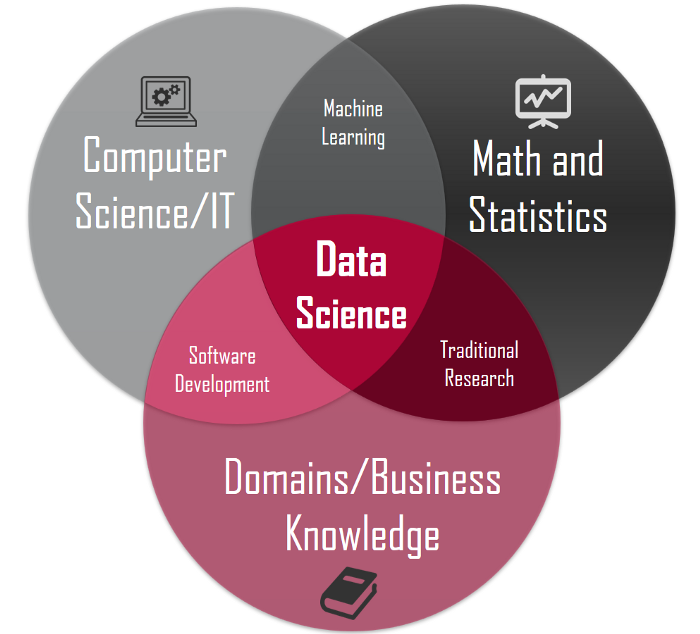
\includegraphics[scale=0.3]{kdd}
			\end{figure}
		\end{frame}
		\begin{frame}{Intención Emprendedora}		
			\begin{figure}
				\centering
				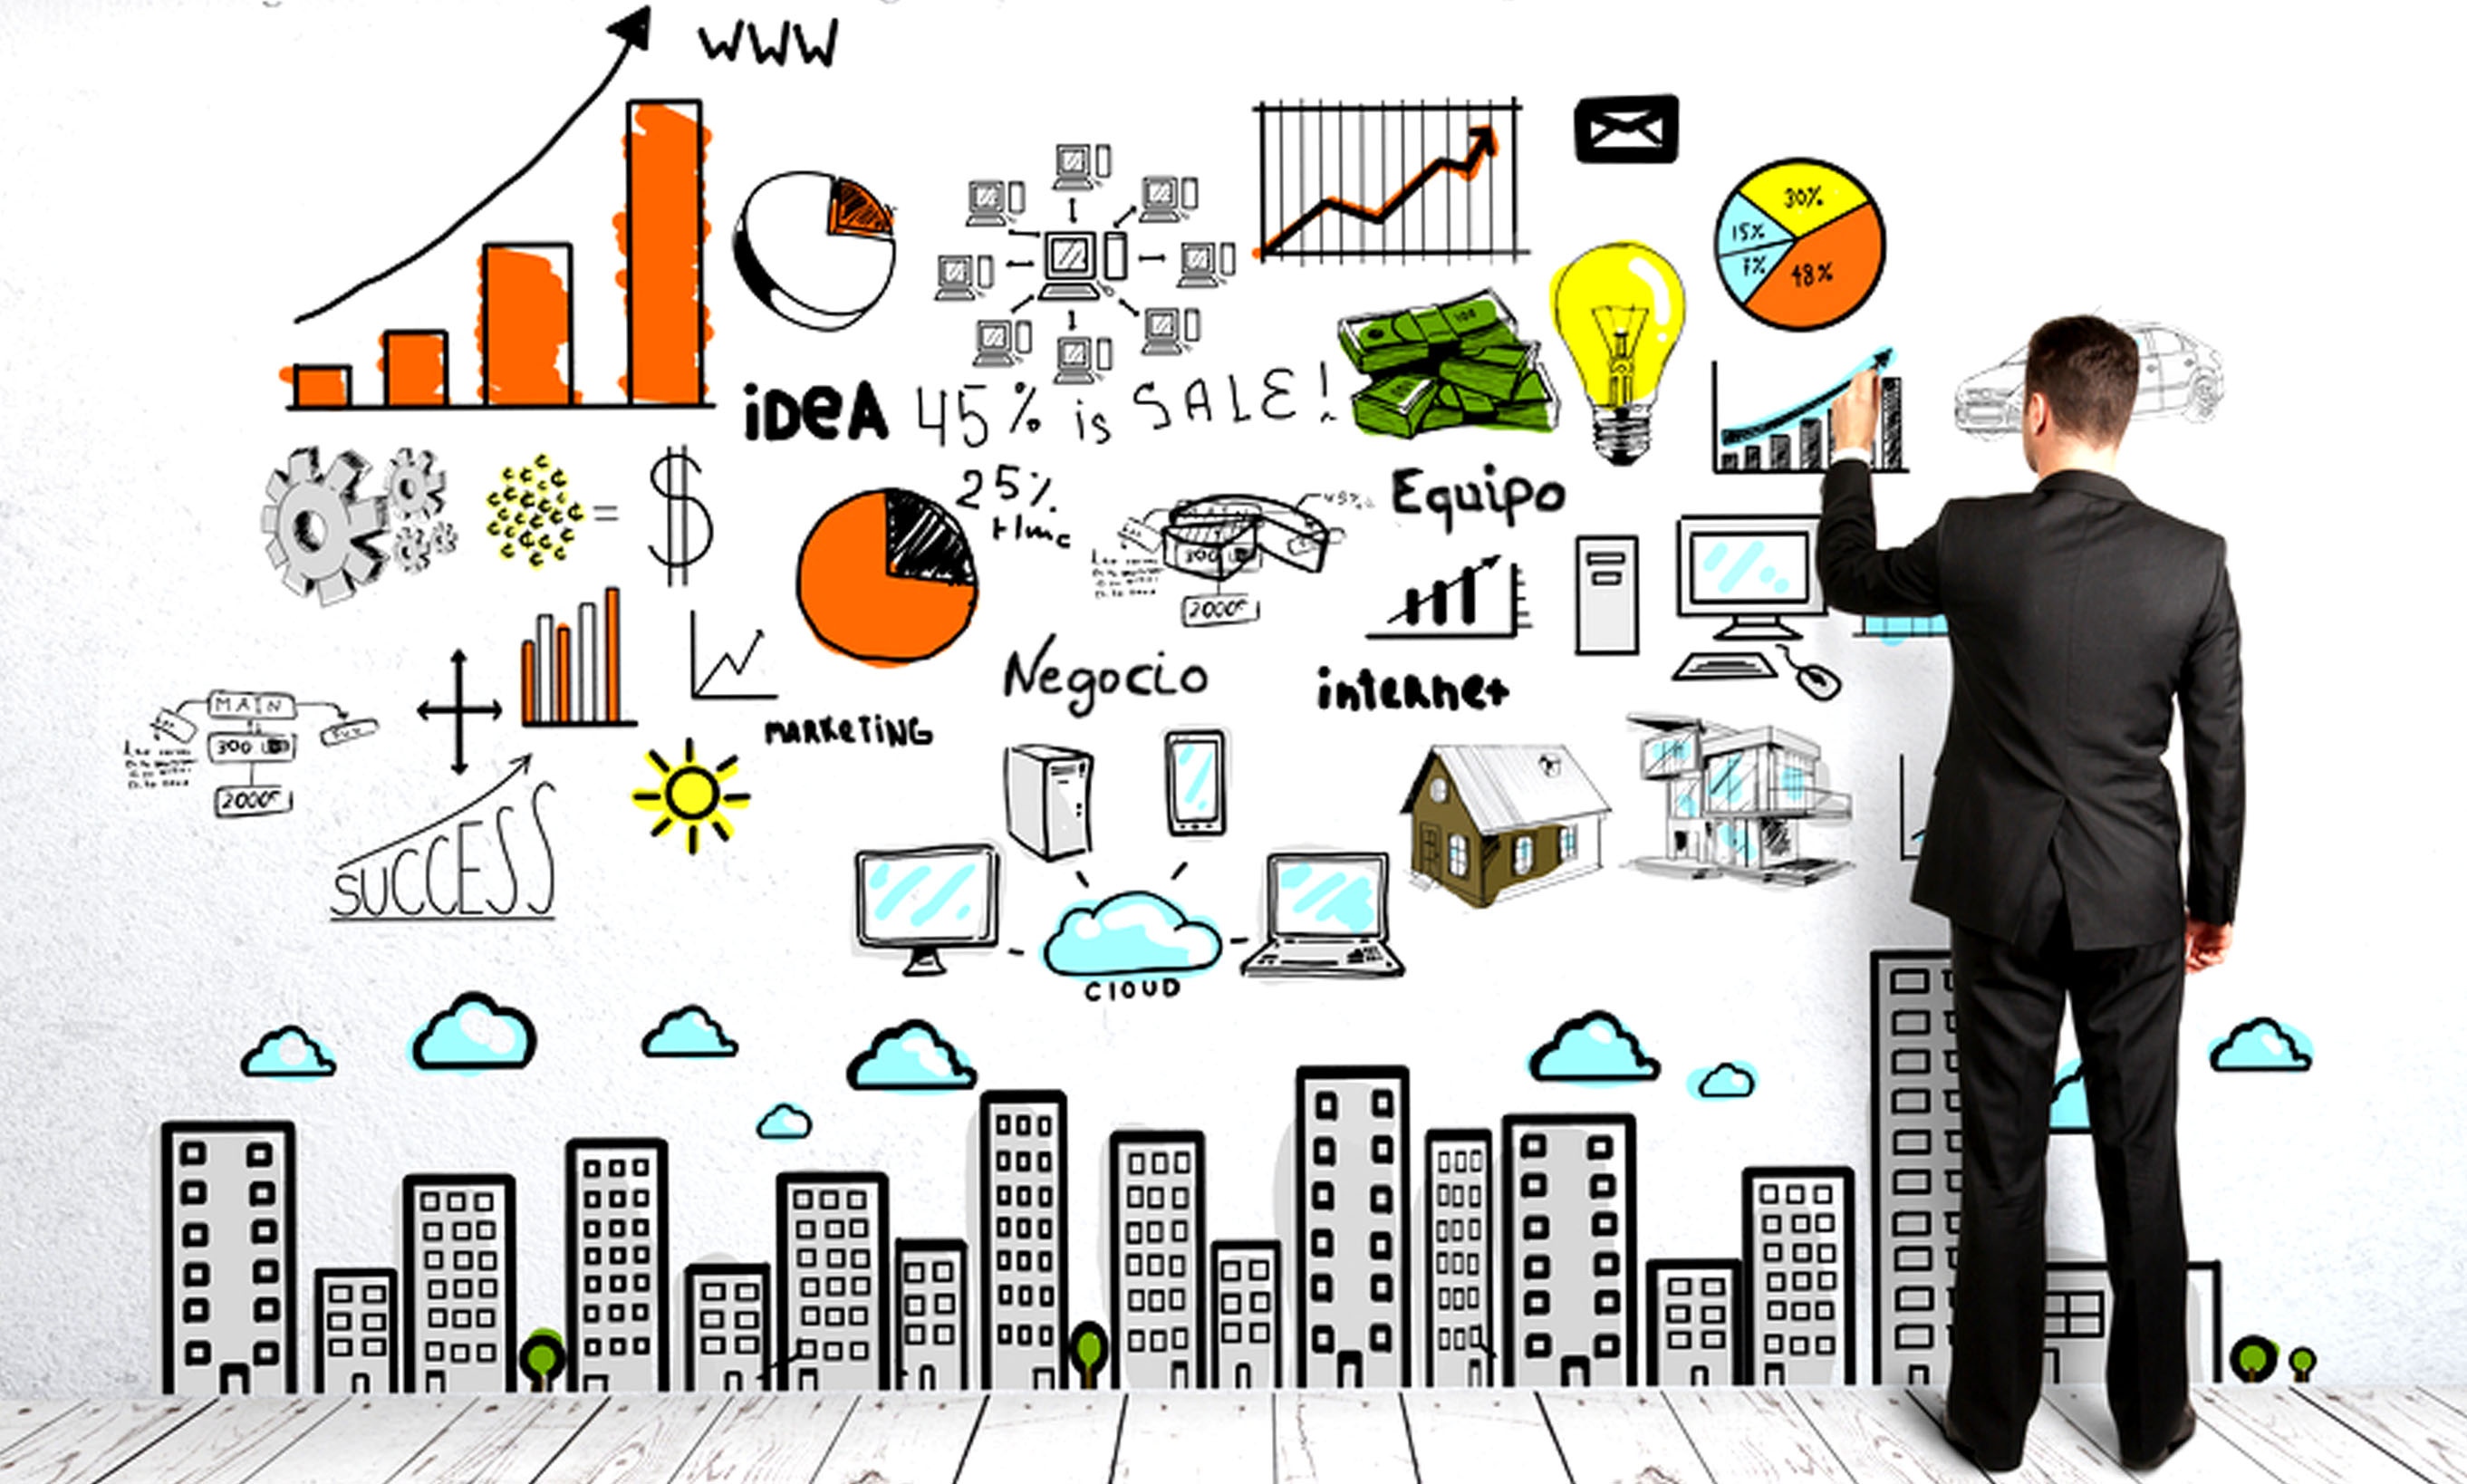
\includegraphics[scale=0.4]{ie}
			\end{figure}
		\end{frame}{}
\section{Problema}
		\subsection{Objetivos}
\begin{frame}{Objetivos del trabajo}
	\begin{itemize}
		\item ¿Hay conocimiento en el conjunto de datos?
		\item ¿Se puede predecir la intención emprendedora?
		\item ¿Cuales son los factores más importantes?
	\end{itemize}
\end{frame}
	\subsection{Descripción}
		\begin{frame}{¿Como se han recogido los datos?}
 			\begin{figure}
			 	\centering
			 	
\includegraphics[scale=0.4]{encuesta}
			 \end{figure}
		\end{frame}
	\begin{frame}{¿Como se han compartido con nosotros?}
 			\begin{figure}
				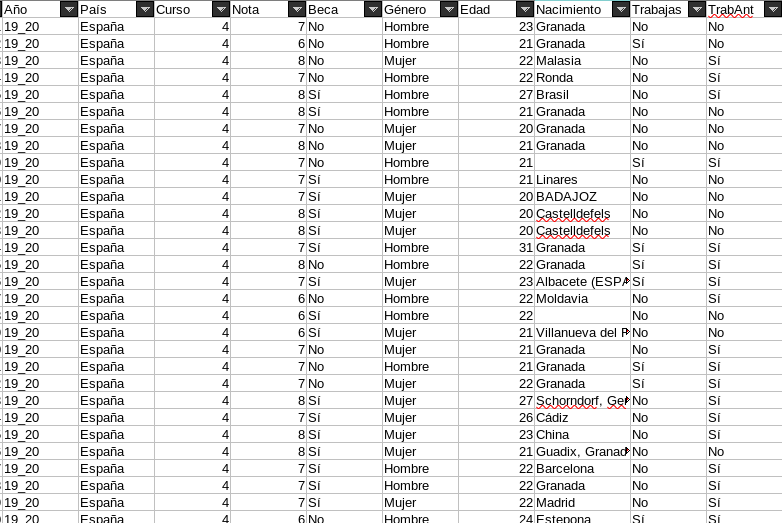
\includegraphics[scale=0.35]{datos}
			\end{figure}
		\end{frame}
	\subsection{Datos}
		\begin{frame}{Variables que forman el conjunto de datos}
			\begin{itemize}
				\item Variables de control. (País, edad, sexo, etc)
				\item Variables de emprendimiento. (Auto-eficacia, actitud y norma social)
				\item Variables de competencias (Conocimientos financieros, auto-evaluación, etc)
				\item Variables de inclusión financiera.
				\item Conocimientos financieros emprendedores (balance, rentabilidad, ventas)
			\end{itemize}
		\end{frame}
		\begin{frame}{Muestra de los datos a predecir}
			\begin{itemize}
				\item \textbf{IE1:} Estoy dispuesto a hacer cualquier cosa para ser un emprendedor.
				\item \textbf{IE2:} Mi objetivo profesional es ser emprendedor.
				\item \textbf{IE3:} Haré todo lo posible para crear y dirigir mi propia empresa.
				\item \textbf{IE4:} Estoy decidido a crear mi propia empresa. 
				\item \textbf{IE5:} He reflexionado seriamente sobre crear una empresa.
				\item \textbf{IE6:} Tengo la firme intención de crear una empresa algún día. 
				\item \textbf{IEMedia:} Media de todos los valores anteriores. 
			\end{itemize}
		Todas estas variables (exceptuando \textit{IEMedia}) están en una escala Likert tomando valores de 1 a 7.
		\end{frame}

\section{Enfoques}
	\subsection{Regresión}
		\begin{frame}{¿En qué consiste la regresión?}
 			\begin{figure}
				\centering
				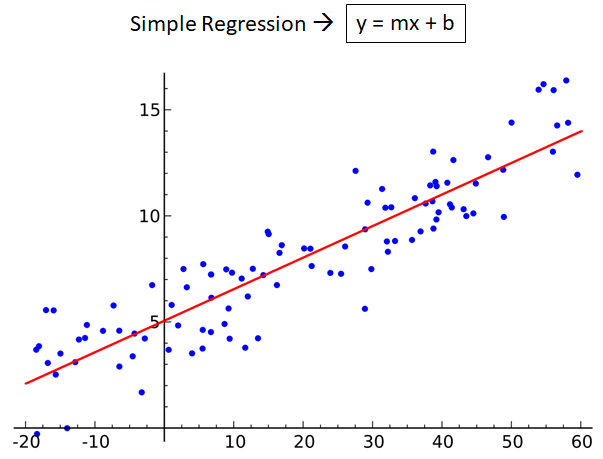
\includegraphics[scale=0.4]{regresion }
			\end{figure}
		\end{frame}
		\begin{frame}{Justificación de este enfoque}
			\begin{itemize}
				\item Existencia de la variable \textit{IEMedia}.
				\item Nos permite identificar cual es la intención emprendedora.
				\item Es un problema clásico de Aprendizaje Automático.
				\item Como primer enfoque, nos sirve para detectar si hay conocimiento o no en el conjunto.
			\end{itemize}
		\end{frame}
		\begin{frame}{Resultados en conjunto de Test}
			\begin{figure}
				\centering
				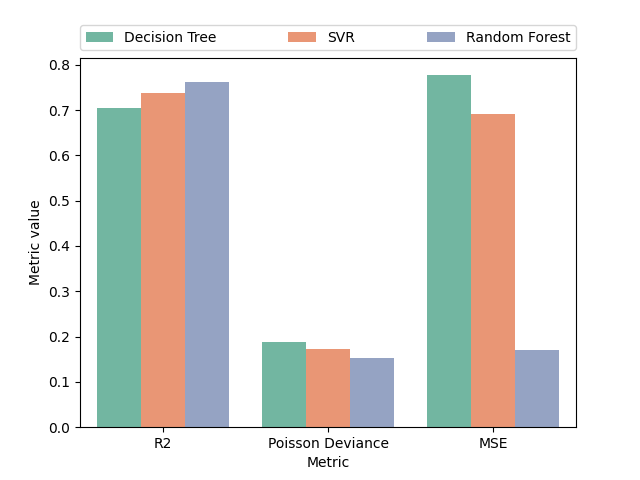
\includegraphics[scale=0.5]{reg_test_metrics}
			\end{figure}
		\end{frame}
	\subsection{Clasificación Ordinal}
		\begin{frame}{¿En qué consiste la clasificación ordinal?}
 			\begin{figure}
				\centering
				
\includegraphics[scale=0.4]{likert}
			\end{figure}
		\end{frame}
		\begin{frame}{Justificación de este enfoque}
			\begin{itemize}
				\item Se está trabajando con datos que facilitan este tipo de clasificación.
				\item Se puede modificar la variable \textit{IEMedia} para usar este enfoque.
				\item Facilitar la accesibilidad para personas no familiarizadas con problemas de regresión.

			\end{itemize}
		\end{frame}
		\begin{frame}{Resultados usando división $(4, 6, 7)$}
			\begin{figure}
				\centering
				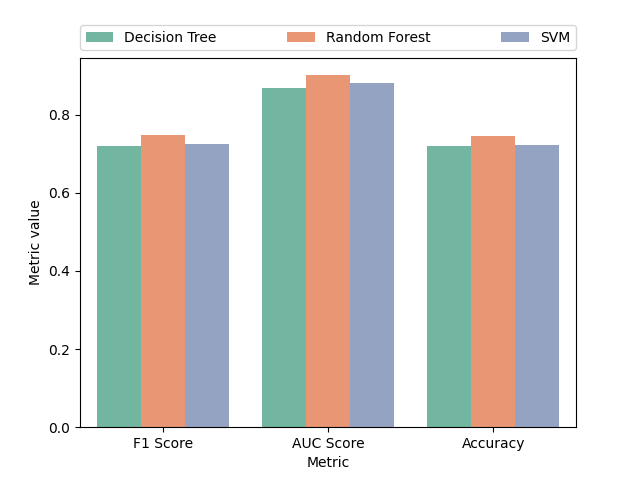
\includegraphics[scale=0.5]{ord_test_metrics}
			\end{figure}
		\end{frame}
	\subsection{Clasificación multi-etiqueta}
		\begin{frame}{¿En qué consiste la clasificación multi-etiqueta?}
 			\begin{figure}
				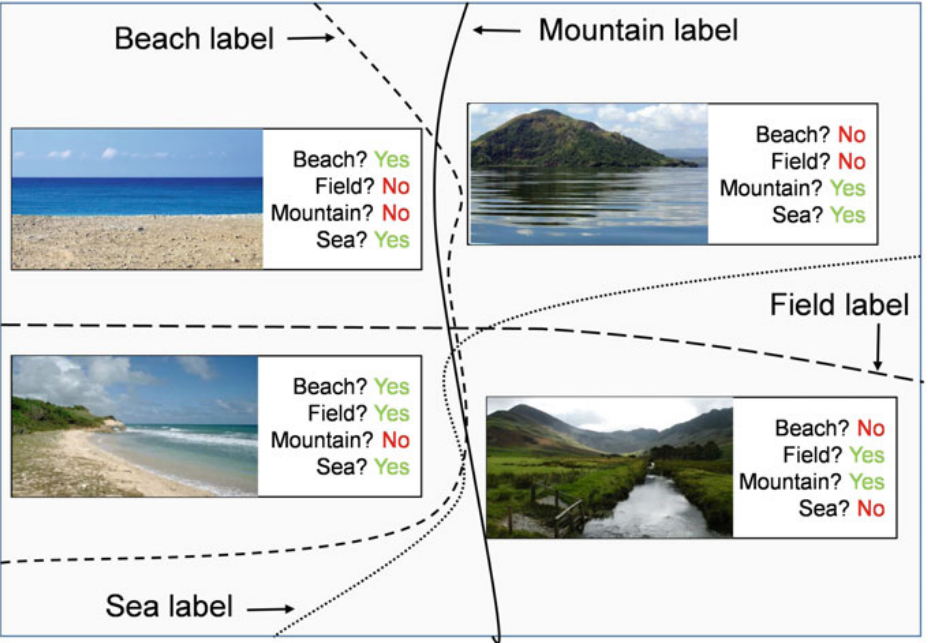
\includegraphics[scale=0.4]{../multilabel-class}
			\end{figure}
		\end{frame}
		\begin{frame}{Justificación de este enfoque}
			\begin{itemize}
				\item El conjunto de datos tiene varias etiquetas para predecir.
				\item Se puede obtener la importancia de las variables que influyen en cada etiqueta.
			\end{itemize}
		\end{frame}
		\begin{frame}{Resultados usando los valores medios calculados por cada etiqueta}
			\begin{figure}
				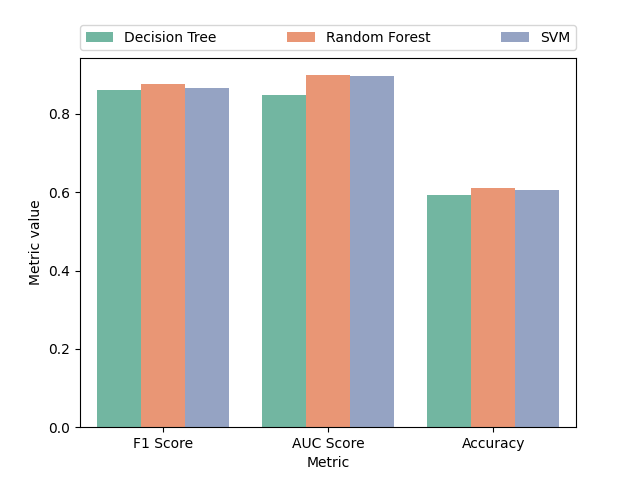
\includegraphics[scale=0.5]{br_test_metrics}
			\end{figure}
		\end{frame}
\section{Conclusiones}
	\subsection{¿Hay conocimiento en el conjunto de datos?}
		\begin{frame}{¡Hay conocimiento en el conjunto de datos!}
			\begin{itemize}
				\item Con los resultados que se ha visto, podemos asegurar que hay conocimiento en el conjunto de datos.
				\item Se puede predecir la Intención emprendedora media, usando regresión, clasificación ordinal.
				\item Podemos predecir cada una  de las etiquetas que se han usado para calcular la intención emprendedora media.
			\end{itemize}
		\end{frame}
	\subsection{¿Cuales son las preguntas más importantes?}
		\begin{frame}{Relevancia de preguntas}
 			\begin{figure}
				\includegraphics[scale=0.5]{../src/dt-br_dt_features}
			\end{figure}
		\end{frame}
\section{Bibliografía}
\begin{frame}{Citas}
	\begin{itemize}
		\item \url{https://towardsdatascience.com/introduction-to-statistics-e9d72d818745}
		\item \url{https://www.diariocritico.com/noticia/497679/emprendedores-2020/nace-el-primer-mapa-del-emprendimiento-social-juvenil-en-espana.html}
		\item \url{https://blogging-techies.com/como-crear-un-cuestionario-a-escala-likert-en-wordpress/}
		\item Francisco Herrera, Francisco Charte, Antonio J. Rivera, María J. del Jesus.
	\end{itemize}
\end{frame}
\end{document}


